%% Street-to-Street Dress Retrieval (ACM sigconf). English source: paper_en.md.
%% Draft: references (paper.bib) are not verified against the original sources.
%% Build: pdflatex paper && bibtex paper && pdflatex paper && pdflatex paper
\documentclass[sigconf,nonacm]{acmart}
\setlength{\emergencystretch}{2em}
\captionsetup[table]{skip=3pt}  % space between a table caption and the table (default 10pt)

%% acmart stops with an error when an affiliation has no \country; for this preprint the check is disabled.
\makeatletter
\def\@ACM@checkaffil{}
\makeatother

%% Preprint: nonacm removes the ACM reference format, copyright block, and conference running heads.

\AtBeginDocument{\providecommand\BibTeX{{Bib\TeX}}}

\begin{document}

\title[Street-to-Street Dress Image Retrieval]{Contrastive Learning Reduces Background Distraction, but Resolution Limits Dress Retrieval}

\author{Sungjin Park}
\affiliation{\institution{KAIST AI}}
\email{sungjin@kaist.ac.kr}

\renewcommand{\shortauthors}{Park}

\begin{abstract}
Retrieving other street photos of the same dress from a street photo is hard because the dress covers only about 20\% of the image, so the background and the wearer dominate general-purpose image embeddings. Explicit grounding, which locates the dress with a bounding box, is a natural remedy. It is unclear, however, whether it is still needed after contrastive training, and whether its benefit comes from removing the background or from higher resolution. We study this on Street2Shop dresses. On an off-the-shelf SigLIP2, cropping the dress raises R@1 from 0.226 to 0.626, and background removal and higher resolution each explain about half of the gain. Training only LoRA adapters contrastively on pairs of photos of the same product reaches an R@1 of 0.870, 0.103 higher than the zero-shot Tianmu-MERE. On this trained model, masking the background and the bounding-box loss no longer help, but enlarging the detected dress region raises R@1 to 0.920, mostly on small dresses. Hence, after contrastive learning, explicit grounding is useful for recovering resolution, not for removing the background. Supplementary materials are provided at \url{https://github.com/sungjin-code/dress-retrieval}.
\end{abstract}

\keywords{Image Retrieval, Contrastive Learning, LoRA, Visual Grounding}

\maketitle

%% ---------------------------------------------------------------- 1
\section{Introduction}

We study retrieval of street photos of the same dress product. The query is a street photo, and the model searches a gallery of street photos. The input is the full, uncropped scene. A gallery photo is correct if it has the same product ID as the query, so correctness depends on product identity, not on style similarity.

A query and its matches share little besides the dress. The wearer, pose, location, and lighting all differ, and the dress covers a median of only 19.6\% of the image. A general-purpose embedding summarizes the whole image in one vector, so the background and the wearer can dominate it. For example, all-against-all retrieval over the 10,124 street photos of dresses in Street2Shop with an off-the-shelf SigLIP2 gives an R@1 of only 0.152 (Figure~\ref{fig:examples}).

\begin{figure}[t]
  \centering
  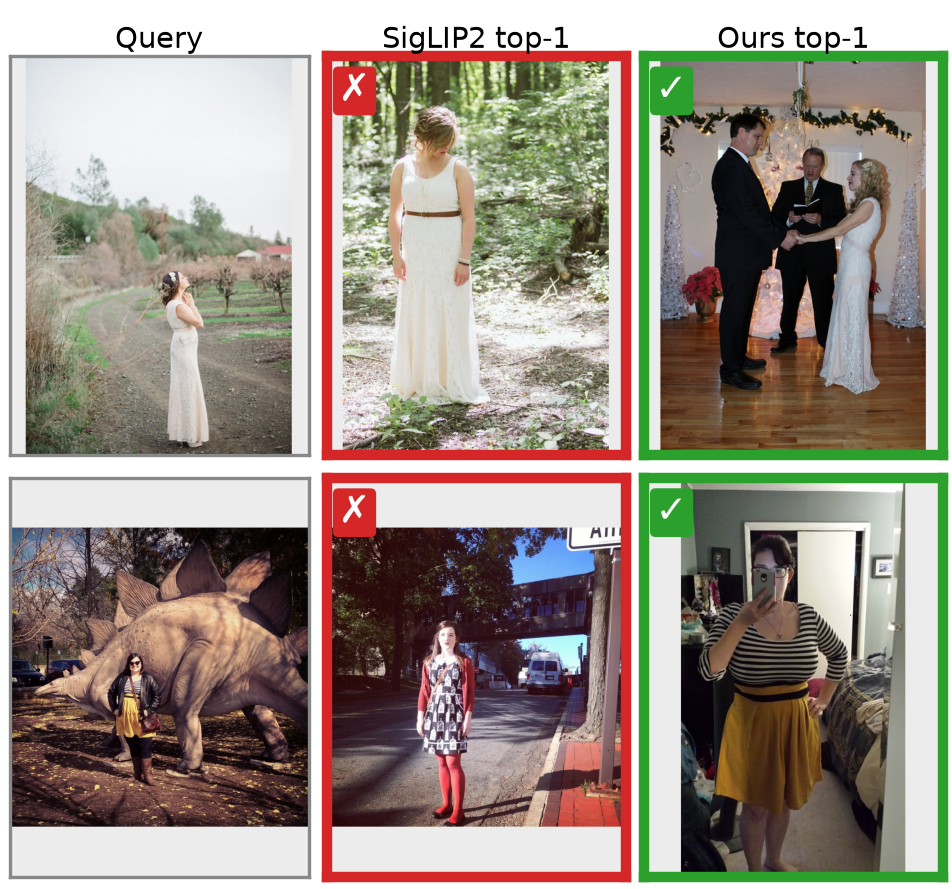
\includegraphics[width=\columnwidth]{fig/fig1_examples.png}
  \caption{Qualitative examples. Each row shows a query street photo, the top-1 result of the off-the-shelf SigLIP2, and the top-1 result of our model. Green frames mark photos of the same product, and red frames mark photos of a different product. The queries were drawn at random from those with small dresses on which SigLIP2 fails and our model succeeds, so the examples are illustrative rather than typical.}
  \Description{Two queries, each with the wrong top-1 result of SigLIP2 and the correct top-1 result of the trained model.}
  \label{fig:examples}
\end{figure}

Prior work on clothing retrieval has mainly addressed retrieving shop photos from street photos~\cite{kiapour2015,liu2016deepfashion,huang2015darn,ge2019deepfashion2}. We study the case where both the query and the gallery are street photos. Both contain backgrounds, so background similarity can easily mislead retrieval. Image-text pretrained encoders such as CLIP~\cite{radford2021clip}, SigLIP~\cite{zhai2023siglip}, and SigLIP~2~\cite{tschannen2025siglip2} are widely used as retrieval backbones, and e-commerce-specific embeddings such as Marqo Ecommerce~\cite{marqo2024} and Tianmu-MERE~\cite{tianmu} are publicly available. We use InfoNCE~\cite{oord2018cpc,chen2020simclr}, replacing the text of each pair with another photo of the same product, and train only LoRA~\cite{hu2022lora} adapters on a frozen backbone.

An intuitive remedy for the background problem is to use the location of the dress explicitly. We call this explicit grounding. We test an auxiliary bounding-box loss during training, and two inputs at inference: cropping the image to a detected box (crop) and masking out everything outside the box (mask). These methods likely help an untrained model. It is unclear whether they are still needed after contrastive learning, and whether their benefit comes from background removal or from higher resolution.

We ask three research questions. RQ1: why do general-purpose image embeddings fail at street-to-street dress retrieval? RQ2: how much does contrastive learning on pairs of photos of the same product fix this, and what drives the improvement? RQ3: does explicit grounding still help a trained model, and does its benefit come from background removal or from higher resolution? Our contributions are:
\begin{enumerate}
  \item We split the failure of the off-the-shelf SigLIP2 into background and resolution effects, and show that they contribute equally.
  \item We show that a small model trained only with LoRA adapters clearly outperforms a large e-commerce embedding model, mainly because of street-photo training data from the same distribution as the test data.
  \item We show that for a trained model, background removal and the bounding-box loss do not help. Only cropping with a detected box helps, and it helps through higher resolution.
\end{enumerate}
RQ1 is addressed in Section~\ref{sec:analysis}, RQ2 in Sections~\ref{sec:results} and~\ref{sec:ablation}, and RQ3 in Sections~\ref{sec:ablation} and~\ref{sec:analysis}.

%% ---------------------------------------------------------------- 2
\section{Method}

\subsection{Problem Definition}

Each street photo $x$ has a product label $y(x)$. An encoder $f$ maps the full photo to an L2-normalized embedding $f(x)$. Given a query $q$, gallery photos $g$ are ranked in descending order of $\cos(f(q), f(g))$. Retrieval is better when photos with $y(g) = y(q)$ are ranked higher.

\subsection{Model Architecture}

The backbone is the vision encoder of SigLIP2-base (\path{google/siglip2-base-patch16-224})~\cite{tschannen2025siglip2}, whose weights are all frozen. LoRA is applied to the attention projections and the MLP layers of every layer ($r = 32$, $\alpha = 64$, dropout $0.3$), giving 5.3M trainable parameters, or 1.4\% of the total. During training, a bounding-box head that predicts the dress box from the patch tokens is attached. At inference, the LoRA weights are merged into the backbone, so the model has the same size and speed as the original SigLIP2 (Figure~\ref{fig:arch}).

\begin{figure}[t]
  \centering
  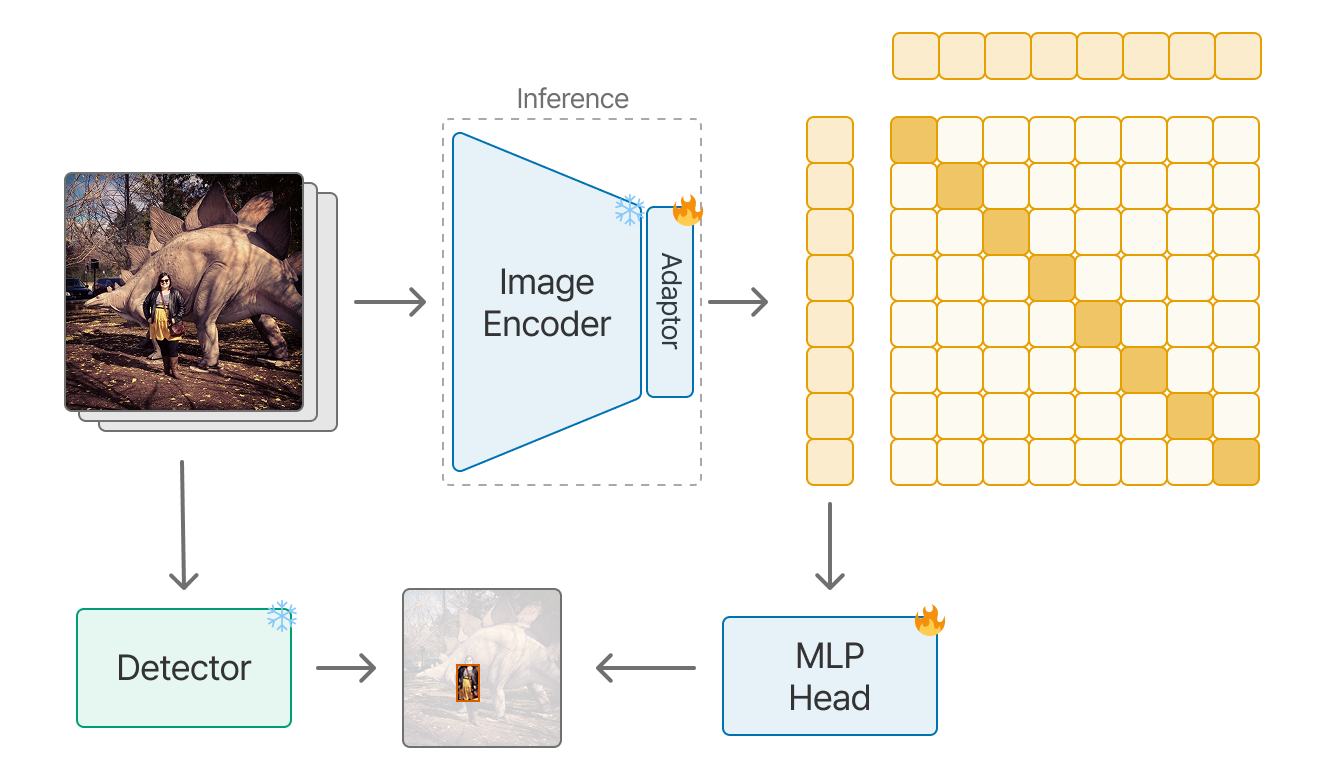
\includegraphics[width=\columnwidth]{fig/fig2.png}
  \caption{Overview of our method. Photos of the same product pass through the frozen SigLIP2 image encoder with trainable LoRA adapters. The embeddings of two photos per product form a similarity matrix, and InfoNCE pulls the matching pairs on the diagonal together. A trainable bounding-box head is supervised by the dress box from a frozen detector or the dataset annotation. Only the encoder with LoRA (dashed box) is used at inference. Snowflakes mark frozen modules and flames mark trained modules.}
  \Description{Diagram of the training pipeline: an image encoder with LoRA adapters produces embeddings, a similarity matrix with a highlighted diagonal defines the contrastive loss, and a bounding-box head and a detector provide the box loss.}
  \label{fig:arch}
\end{figure}

\subsection{Training Objective}

Each batch consists of $P$ distinct products, and two different photos are sampled for each product. Letting $\mathbf{a}_i$ and $\mathbf{b}_i$ denote the embeddings of the two photos of product $i$, the objective is
\begin{align}
  \mathcal{L} &= \mathcal{L}_{\mathrm{cont}} + \lambda \mathcal{L}_{\mathrm{bbox}}, \\
  \mathcal{L}_{\mathrm{cont}} &= \tfrac{1}{2}\left(\operatorname{CE}(S, y) + \operatorname{CE}(S^{\top}, y)\right), \qquad
  S_{ij} = \frac{\cos(\mathbf{a}_i, \mathbf{b}_j)}{\tau},
\end{align}
where $y = (0, \ldots, P-1)$, so that all photos of other products in the batch serve as negatives. $\mathcal{L}_{\mathrm{bbox}}$ is the sum of the L1 loss and the GIoU loss~\cite{rezatofighi2019giou} between the predicted and ground-truth boxes. We set $\lambda = 0.3$ and $\tau = 0.05$. The bounding-box loss is explicit grounding during training. It encourages the encoder to attend to the dress.

\subsection{Training Procedure}

Training proceeds in two stages. We first pretrain from the off-the-shelf SigLIP2 on shop photos. Shop photos have simple backgrounds and show the dress large, so this stage teaches the model to tell dresses apart. Shop photos have no ground-truth boxes, so we use boxes detected by OWLv2~\cite{minderer2023owlv2} as targets. We then train on street photos, using the product boxes provided by the dataset. In both stages, checkpoints are selected by R@1 on the street-photo validation set. To make the model robust to lighting, we apply color jitter (brightness, contrast, and saturation, each 0.6) to each training image independently.

\subsection{Input Transformations at Inference}

We keep the trained model fixed and change only its input. \emph{Crop} cuts the photo to the dress box and resizes it to 224 px, so it removes the background and raises the resolution. \emph{Mask} removes everything outside the box but keeps the photo size, so it removes only the background. To check the effect of the fill, we fill the outside of the box in three ways: white, the image mean color, or a blurred copy of the image. The \emph{background-only} input does the opposite: it erases the dress by filling the inside of the box. Crop and mask differ only in resolution, so comparing them splits the effect of cropping into background removal and higher resolution.

For the analysis, we use OWLv2 boxes so that every model gets the same boxes. For our model we also evaluate two-pass inference with the boxes predicted by its own bounding-box head. The same transformation is applied to both queries and gallery images.

%% ---------------------------------------------------------------- 3
\section{Experiments}

\subsection{Dataset}

We use the \texttt{dresses} category of Street2Shop~\cite{kiapour2015}, taken from a Hugging Face mirror (\path{petr7555/street2shop})~\cite{street2shopmirror} with product IDs and product boxes (Appendix~\ref{app:data}). We exclude 95 photos that contain more than one product, because their labels are ambiguous.

From the 1,792 products with at least two photos, we randomly select 200 products for validation and 300 for testing, and use the remainder for training (Table~\ref{tab:data}). In the test set, half of each product's photos serve as queries and the rest as gallery images. Shop photos are used only for pretraining, and shop photos of validation and test products are excluded. No product appears in more than one split.

\begin{table}[t]
  \caption{Dataset composition.}
  \label{tab:data}
  \small
  \begin{tabular}{lrrr}
    \toprule
    Split & Products & Photos & SigLIP2 R@1 \\
    \midrule
    Street, train & 3,701 & 7,930 & -- \\
    Street, validation & 200 & 879 & 0.291 \\
    Street, test & 300 & 1,315 & 0.226 \\
    Shop (pretraining) & 3,776 & 15,891 & -- \\
    \bottomrule
  \end{tabular}
  \par\smallskip
  %\footnotesize The test photos comprise 716 queries and 599 gallery photos. SigLIP2 is the off-the-shelf model.
\end{table}

\subsection{Experimental Setup}

\paragraph{Evaluation.} For each query, we compute cosine similarity to the entire gallery by exact search and report R@K and nDCG@5. R@K is the fraction of queries for which a photo of the same product appears among the top $K$ results. The R@1 of a random ranking is 0.007. We call a difference between models significant if the 95\% confidence interval of a paired bootstrap over queries~\cite{efron1993bootstrap} (5,000 resamples) excludes zero. This interval reflects only the sampling variation of test queries, so we measure variation across training seeds separately by training our model with three seeds.

\paragraph{Training.} We use AdamW (weight decay 0.3), a cosine schedule, and bf16 precision. Training runs for at most 20 epochs and stops when validation R@1 has not improved for 5 consecutive epochs. Hyperparameters are selected on validation R@1 only (learning rate $2\times10^{-5}$ and batches of 32 products, see Appendix~\ref{app:hp}), and the test set is used only after selection. Additional results and the full training configuration are given in Appendices~\ref{app:extra} and~\ref{app:config}.

\paragraph{Compared models.} We compare against the untrained off-the-shelf SigLIP2 and two zero-shot e-commerce embeddings, Marqo Ecommerce~\cite{marqo2024} and Tianmu-MERE~\cite{tianmu}. Each ablation changes a single component of our model. The variants are a model with shop pretraining only, a model without color jitter, a model without the bounding-box loss in the street stage, and a model with street training only.

\subsection{Results}
\label{sec:results}

\begin{table}[tb]
  \caption{Comparison with existing models.}
  \label{tab:main}
  \small
  \resizebox{\columnwidth}{!}{%
  \begin{tabular}{lrrrrr}
    \toprule
    Model & Input & R@1 & R@5 & R@10 & nDCG@5 \\
    \midrule
    SigLIP2 & 224 & 0.226 & 0.415 & 0.503 & 0.212 \\
    Marqo Ecommerce & 224 & 0.380 & 0.550 & 0.616 & 0.344 \\
    Tianmu-MERE & 384 & 0.767 & 0.869 & 0.901 & 0.737 \\
    Ours & 224 & \textbf{0.870} & \textbf{0.948} & \textbf{0.968} & \textbf{0.874} \\
    \bottomrule
  \end{tabular}%
  }
\end{table}

Our model achieves an R@1 of 0.870, exceeding the off-the-shelf SigLIP2 by 0.644 and Tianmu-MERE by 0.103 (Table~\ref{tab:main}). Our model has about one third of the parameters of Tianmu-MERE (375M versus 1,239M) and a lower input resolution. Tianmu-MERE is evaluated zero-shot, so the gap shows the effect of task-specific training, not that one model is better in general. Marqo Ecommerce, trained mainly on shop photos, reaches an R@1 of only 0.380. E-commerce training alone does not transfer well to street photos.

\subsection{Ablation Study}
\label{sec:ablation}

\begin{table}[t]
  \caption{Ablation of training components.}
  \label{tab:ablation}
  \small
  \begin{tabular}{lrrrr}
    \toprule
    Model & R@1 & R@5 & nDCG@5 \\
    \midrule
    Ours & \textbf{0.870} & 0.948 & \textbf{0.874} \\
    w/o street training & 0.800 & 0.905 & 0.801 \\
    w/o color jitter & 0.856 & \textbf{0.954} & 0.867 \\
    w/o bounding-box loss & 0.863 & 0.953 & \textbf{0.874} \\
    w/o pretraining & 0.869 & 0.947 & 0.868 \\
    \bottomrule
  \end{tabular}
\end{table}

Removing street training is the only change with a significant effect (Table~\ref{tab:ablation}). Removing any other component changes R@1 by at most 0.014, within the range of R@1 from retraining the same configuration with different seeds (Table~\ref{tab:seeds}).

\paragraph{Street training.} A model trained only on shop photos, without a single street photo, already reaches an R@1 of 0.800, matching or exceeding Tianmu-MERE. Pulling photos of the same product together seems enough to learn the color, pattern, and shape of the dress, and this transfers to photos with backgrounds. Street training adds 0.070 in R@1, more on small dresses (Tables~\ref{tab:size} and~\ref{tab:d2}). Handling small dresses against a background seems to be learned from data of the evaluation distribution.

\paragraph{Auxiliary bounding-box loss.} Removing the bounding-box loss from the street stage changes R@1 by less than 0.01 (0.863 versus 0.870), and R@5 is slightly higher without it. The shop pretraining stage still uses the loss. We find no evidence that the bounding-box loss improves retrieval. A likely reason is that contrastive learning already directs attention to the dress, the part shared by photos of the same product, so localization supervision adds little. The results in Section~\ref{sec:analysis} support this.

\paragraph{Color jitter and pretraining.} Removing color jitter lowers R@1 but raises R@5, so we find no evidence that it improves robustness to lighting. Shop pretraining does not change final performance (R@1 0.869 without it versus 0.870).

\subsection{Analysis of Cropping and Masking}
\label{sec:analysis}

All analyses in this section use the full test set, with the same OWLv2 boxes for every model (Tables~\ref{tab:input} and~\ref{tab:size}). Figure~\ref{fig:inputs} gives a qualitative example.

\begin{table}[t]
  \caption{R@1 by input type.}
  \label{tab:input}
  \small
  \begin{tabular}{lrrr}
    \toprule
    Input & SigLIP2 & Shop-only & Ours \\
    \midrule
    Original & 0.226 & 0.800 & 0.870 \\
    Mask (white) & 0.418 & 0.763 & 0.821 \\
    Mask (mean color) & 0.426 & 0.774 & 0.823 \\
    Mask (blur) & 0.409 & 0.756 & 0.821 \\
    Crop & 0.626 & 0.873 & \textbf{0.920} \\
    Background only & 0.047 & 0.050 & 0.046 \\
    \bottomrule
  \end{tabular}
\end{table}

\begin{table}[t]
  \caption{R@1 by dress size. Queries are divided into tertiles by the fraction of the photo occupied by the product box (small: below 15.6\%, large: 25.1\% or more).}
  \label{tab:size}
  \small
  \setlength{\tabcolsep}{3pt}
  \begin{tabular}{llrrr}
    \toprule
    Model & Input & Small & Medium & Large \\
    \midrule
    SigLIP2 & Original & 0.172 & 0.238 & 0.268 \\
    SigLIP2 & Mask (white) & 0.307 & 0.435 & 0.510 \\
    SigLIP2 & Crop & 0.605 & 0.611 & 0.661 \\
    Ours & Original & 0.807 & 0.870 & 0.933 \\
    Ours & Mask (white) & 0.731 & 0.824 & 0.908 \\
    Ours & Crop & \textbf{0.908} & \textbf{0.895} & \textbf{0.958} \\
    \bottomrule
  \end{tabular}
\end{table}

\begin{figure*}[t]
  \centering
  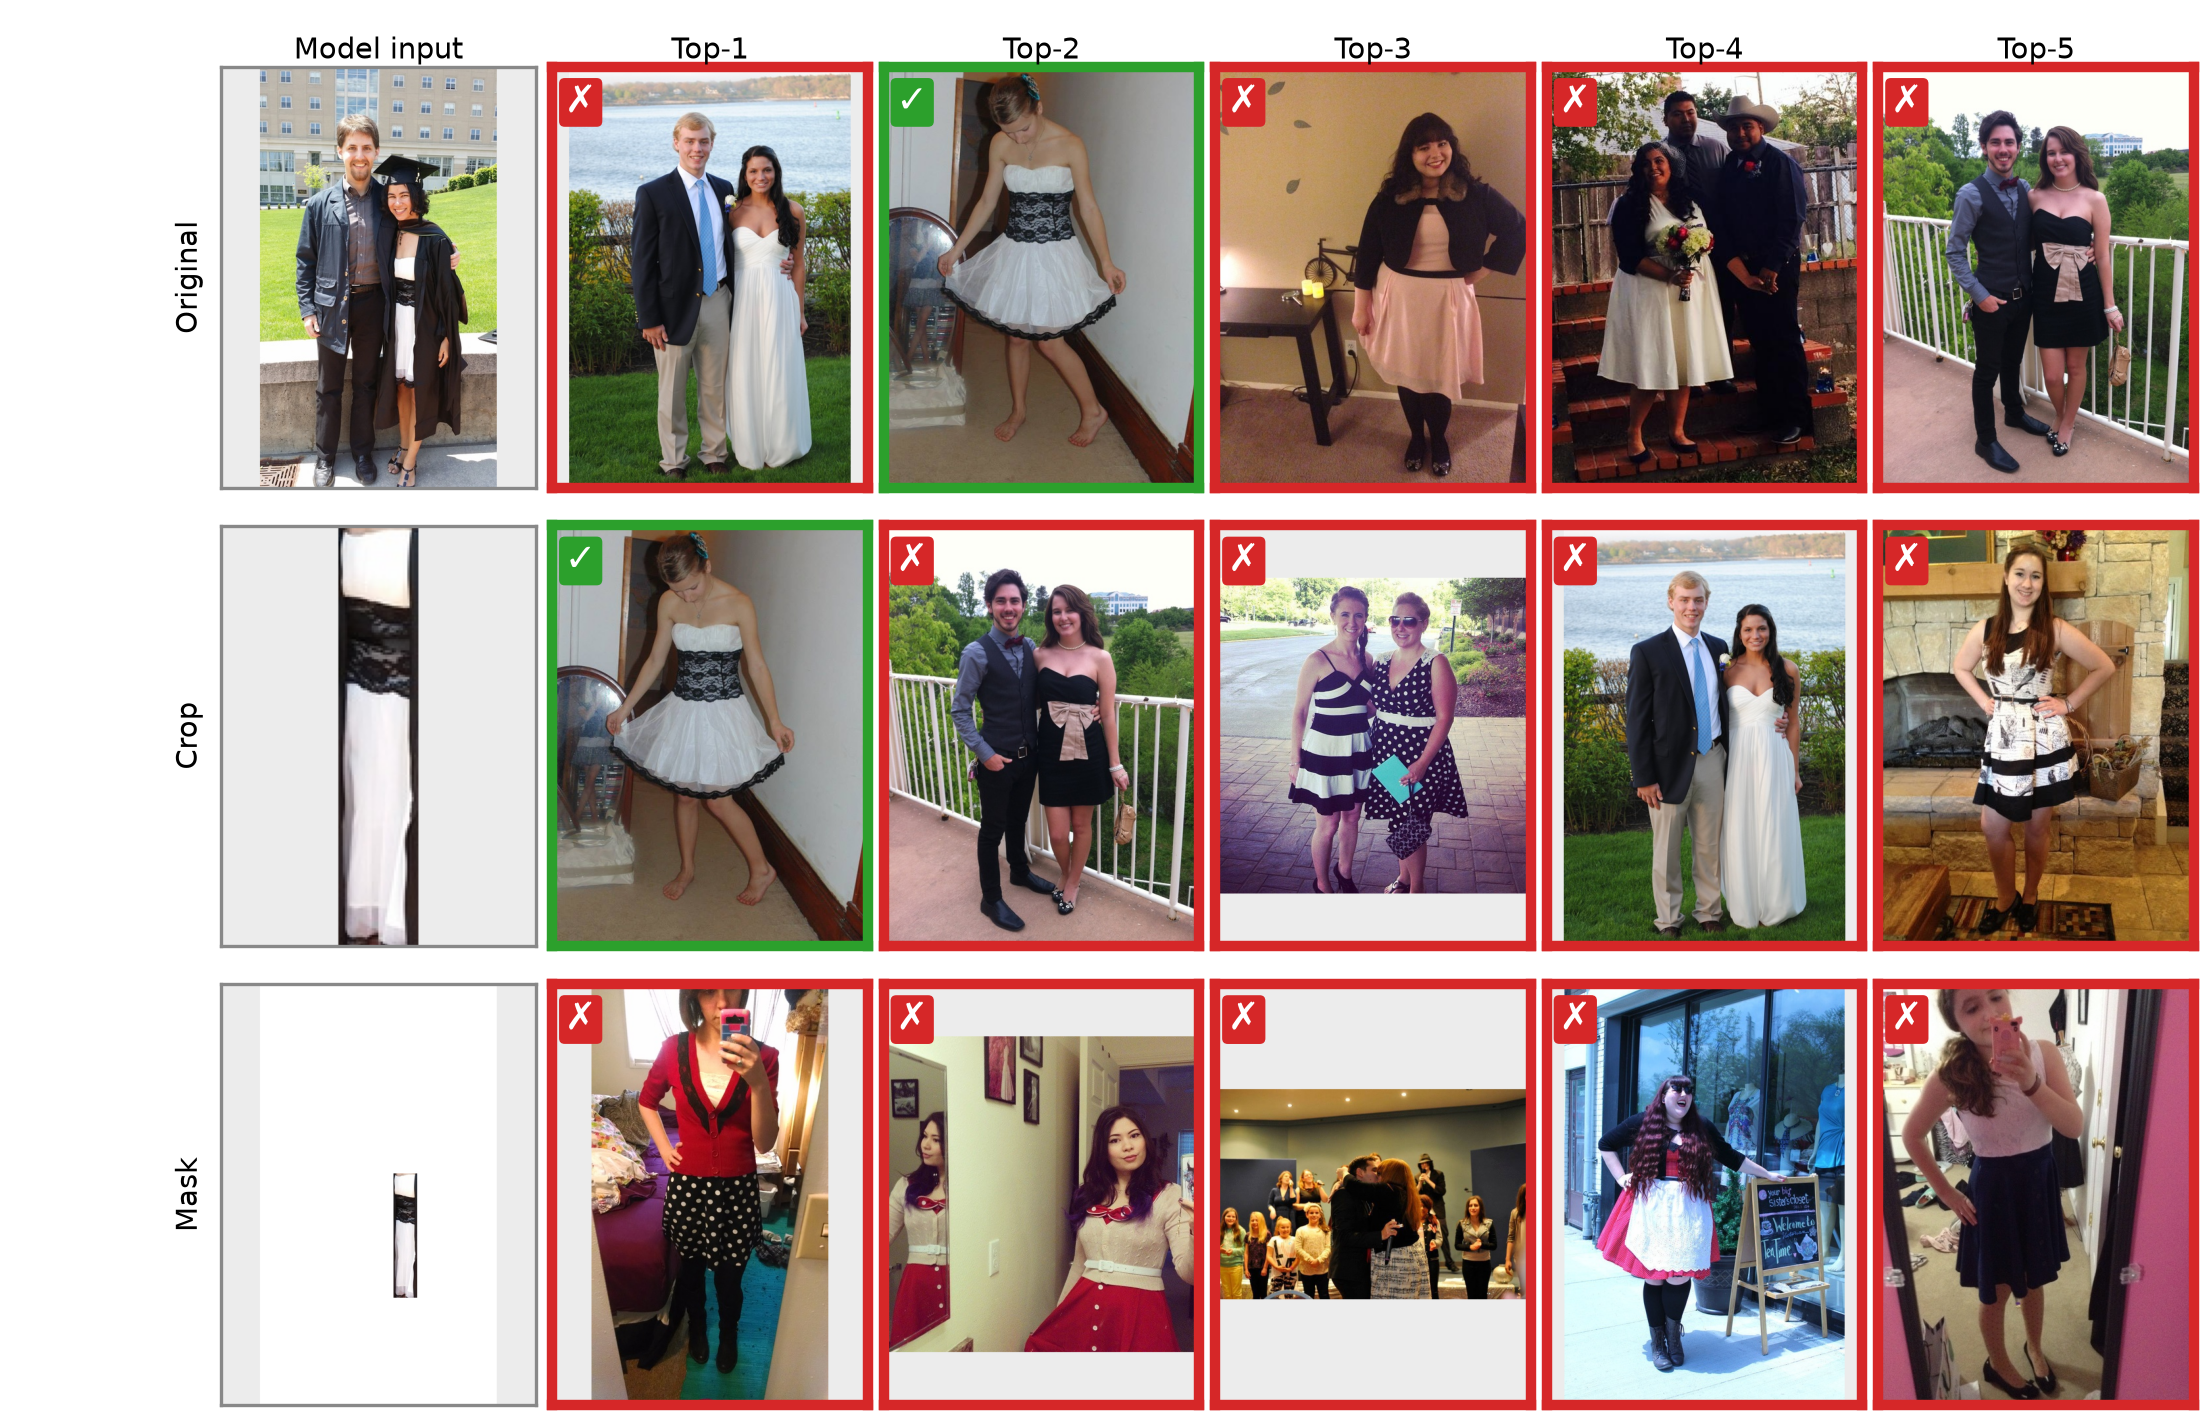
\includegraphics[width=\textwidth]{fig/fig3_inputs.png}
  \caption{One query under the three inputs of Section~\ref{sec:analysis}. The first column is what the model sees. The other columns are the top-5 results of our model for that input (green: same product, red: different product). The query, whose dress covers a small part of the photo, was drawn at random from those on which our model fails on the original photo, succeeds with crop, and fails with mask.}
  \Description{One query under original, crop, and mask inputs, with the top five retrieved photos for each.}
  \label{fig:inputs}
\end{figure*}

\paragraph{Untrained model (RQ1).} Feeding only the dress region to the off-the-shelf SigLIP2 raises R@1 from 0.226 to 0.626. The model and input size are unchanged, so the model does not fail because it cannot tell dresses apart. It fails because information outside the dress dominates the embedding. Masking removes the background and keeps the resolution. It raises R@1 by about 0.19 for every fill, roughly half of the 0.399 gain from cropping. The other half comes from higher resolution. By dress size, background removal helps more for large dresses and higher resolution helps more for small dresses (Table~\ref{tab:size}).

With background-only inputs, R@1 drops to about 0.05 for every model. Two street photos of the same product share almost no background, so the background is not a cue for the match. It is a distractor that pulls in photos of other products.

\paragraph{Trained models (RQ3).} For trained models, background removal no longer helps. Masking raises the R@1 of the off-the-shelf model by 0.19 but lowers that of our model by 0.049. The drop is the same with a blur fill, which keeps natural-image statistics, so the unfamiliar white region alone does not explain it. The trained model seems no longer distracted by the background. It likely uses the parts of the dress, or the way it is worn, that lie outside the box. The shop-only model, which has never seen a street photo, shows the same pattern. So the ability to ignore the background seems to come from contrastive learning itself.

Cropping still helps trained models. Cropping with OWLv2 boxes raises the R@1 of our model to 0.920, a gain of 0.050. Compared with masking with the same boxes, the difference is 0.099, so the gain comes from higher resolution. The gain is largest on small dresses, where R@1 rises from 0.807 to 0.908. With boxes from our own bounding-box head, cropping gives an R@1 of 0.888, a gain that is not significant. The benefit of cropping thus depends on box accuracy.

In summary, the remaining errors come from resolution, not from the background. The input is resized to $224\times224$, so a dress covering less than 15\% of the image gets no more pixels than an $87\times87$ px square.

%% ---------------------------------------------------------------- 4
\section{Conclusion}

We studied why general-purpose image embeddings fail at street-to-street dress retrieval, and what explicit grounding adds after contrastive learning. The failure comes from the background and the wearer dominating the embedding. When only the dress region is given, background removal and higher resolution contribute equally to the gain (RQ1). A model with LoRA adapters trained contrastively on pairs of photos of the same product reaches an R@1 of 0.870, 0.103 higher than Tianmu-MERE. After shop pretraining, the main source of further gain is street-photo data from the evaluation distribution (RQ2). For trained models, background removal and the bounding-box loss do not help. Only cropping with an accurate detected box raises R@1, to 0.920, through higher resolution (RQ3).

After contrastive learning, explicit grounding is useful for recovering resolution for small dresses, not for removing the background. For street-photo retrieval, it is therefore better to collect pairs of street photos of the same product and to give the dress more pixels, by detection-based cropping or higher-resolution input, than to add bounding-box supervision.

The data were split randomly by product, so photos from the same seller may appear in both training and test sets, and detection-based cropping requires a separate detector at inference. Future work will use seller-level splits and compare higher-resolution inputs with training on cropped regions.

%% ---------------------------------------------------------------- refs
\bibliographystyle{ACM-Reference-Format}
\bibliography{paper}

%% ---------------------------------------------------------------- appendix
\appendix

\section{Hyperparameter Search and Seed Repetitions}
\label{app:hp}

We varied one value at a time in the street training stage, starting from the baseline (Table~\ref{tab:hp}), and selected the configuration with the highest validation R@1 as our model.

\begin{table}[ht]
  \caption{Hyperparameter search for the street training stage.}
  \label{tab:hp}
  \small
  \begin{tabular}{lrrrr}
    \toprule
    Configuration & lr & $\tau$ & Batch & Val. R@1 (epoch) \\
    \midrule
    Baseline & $5\times10^{-5}$ & 0.05 & 24 & 0.8680 (4) \\
    Lower lr & $2\times10^{-5}$ & 0.05 & 24 & 0.8714 (11) \\
    Higher $\tau$ & $2\times10^{-5}$ & 0.1 & 24 & 0.8578 (4) \\
    Larger batch (ours) & $2\times10^{-5}$ & 0.05 & 32 & \textbf{0.8726} (6) \\
    \bottomrule
  \end{tabular}
  \par\smallskip
  \footnotesize Batch is the number of products per batch. Val. R@1 is the best value over epochs.
\end{table}

We trained the street stage of our model three times, varying only the seed (Table~\ref{tab:seeds}). The results reported in the main text are for seed 42.

\begin{table}[ht]
  \caption{Performance of our model by seed.}
  \label{tab:seeds}
  \small
  \begin{tabular}{lrrrrr}
    \toprule
    Seed & Val. R@1 & R@1 & R@5 & R@10 & nDCG@5 \\
    \midrule
    42 & 0.8726 & 0.870 & 0.948 & 0.968 & 0.874 \\
    43 & 0.8737 & 0.872 & 0.955 & 0.975 & 0.878 \\
    44 & 0.8692 & 0.860 & 0.947 & 0.969 & 0.864 \\
    Mean & 0.8718 & 0.867 & 0.950 & 0.971 & 0.872 \\
    \bottomrule
  \end{tabular}
\end{table}

The largest R@1 difference between seeds is 0.012, comparable to the differences caused by removing color jitter, the bounding-box loss, or pretraining (0.001--0.014). For some metrics, the paired-bootstrap confidence intervals of the differences between seeds exclude zero. So differences of about 0.01 cannot be attributed to training components.

\section{Data Collection and Statistics}
\label{app:data}

The original Street2Shop repository (\path{lorenzo-stacchio/Street2Shop-Dataset}) provides only lists of image URLs, and the domains hosting the images are no longer reachable. We therefore used the Hugging Face mirror (\path{petr7555/street2shop}). Its product and image IDs form a subset of the original ones, but its source and license are not stated. All photos were stored with their longer side resized to 640 px (Table~\ref{tab:stats}).

\begin{table}[ht]
  \caption{Detailed dataset statistics.}
  \label{tab:stats}
  \footnotesize
  \setlength{\tabcolsep}{3pt}
  \begin{tabular}{lrr}
    \toprule
    Item & Street photos & Shop photos \\
    \midrule
    Photos / products & 10,124 / 4,201 & 18,009 / 4,276 \\
    Photos per product (mean, median) & 2.41, 1 & 4.21, 4 \\
    Median stored resolution & $480\times640$ & $448\times640$ \\
    Median box-area fraction & 0.196 & 0.614 \\
    Box source & Dataset annotation & OWLv2 detection \\
    \bottomrule
  \end{tabular}
\end{table}

\section{Additional Results}
\label{app:extra}

This appendix reports only the models and metrics that do not appear in the main-text tables (Tables~\ref{tab:d1}--\ref{tab:d3}).

\begin{table}[ht]
  \caption{Models not reported in the main text.}
  \label{tab:d1}
  \small
  \setlength{\tabcolsep}{3pt}
  \begin{tabular}{lrrrr}
    \toprule
    Model & R@1 & R@5 & R@10 & nDCG@5 \\
    \midrule
    Ours, crop (bounding-box head) & 0.888 & 0.947 & 0.965 & 0.888 \\
    Ours, mask (bounding-box head) & 0.817 & 0.922 & 0.950 & 0.814 \\
    \bottomrule
  \end{tabular}
\end{table}

\begin{table}[ht]
  \caption{R@1 by dress size for models not reported in Table~\ref{tab:size}.}
  \label{tab:d2}
  \small
  \begin{tabular}{lrrr}
    \toprule
    Model & Small & Medium & Large \\
    \midrule
    Marqo Ecommerce & 0.273 & 0.377 & 0.490 \\
    Tianmu-MERE & 0.672 & 0.778 & 0.849 \\
    w/o street training & 0.718 & 0.791 & 0.891 \\
    w/o color jitter & 0.803 & 0.858 & 0.908 \\
    w/o bbox loss (street stage) & 0.790 & 0.870 & 0.929 \\
    w/o pretraining & 0.786 & 0.866 & 0.954 \\
    Ours, crop (bbox head) & 0.836 & 0.887 & 0.941 \\
    Ours, mask (bbox head) & 0.735 & 0.820 & 0.895 \\
    \bottomrule
  \end{tabular}
  \par\smallskip
  \footnotesize Size tertiles are defined as in Table~\ref{tab:size}, and bbox means bounding-box.
\end{table}

\begin{table}[ht]
  \caption{R@5, R@10, and nDCG@5 by input type. R@1 is reported in Table~\ref{tab:input}.}
  \label{tab:d3}
  \small
  \begin{tabular}{llrrr}
    \toprule
    Model & Input & R@5 & R@10 & nDCG@5 \\
    \midrule
    SigLIP2 & Mask (white) & 0.628 & 0.697 & 0.401 \\
    SigLIP2 & Mask (mean color) & 0.628 & 0.689 & 0.399 \\
    SigLIP2 & Mask (blur) & 0.609 & 0.677 & 0.379 \\
    SigLIP2 & Crop & 0.792 & 0.830 & 0.591 \\
    SigLIP2 & Background only & 0.115 & 0.168 & 0.052 \\
    Shop-only & Mask (white) & 0.880 & 0.915 & 0.750 \\
    Shop-only & Mask (mean color) & 0.888 & 0.919 & 0.762 \\
    Shop-only & Mask (blur) & 0.877 & 0.915 & 0.749 \\
    Shop-only & Crop & 0.944 & 0.951 & 0.864 \\
    Shop-only & Background only & 0.099 & 0.138 & 0.045 \\
    Ours & Mask (white) & 0.912 & 0.932 & 0.813 \\
    Ours & Mask (mean color) & 0.918 & 0.941 & 0.819 \\
    Ours & Mask (blur) & 0.918 & 0.940 & 0.816 \\
    Ours & Crop & 0.958 & 0.958 & 0.902 \\
    Ours & Background only & 0.092 & 0.141 & 0.045 \\
    \bottomrule
  \end{tabular}
\end{table}

The quality of the OWLv2 boxes was assessed on a preliminary sample of 100 test queries and the full gallery (699 images in total). Their IoU with the human-annotated boxes was 0.749 on average and 0.822 at the median, and on the same sample, cropping with ground-truth boxes and cropping with OWLv2 boxes yielded the same R@1 of 0.64.

\section{Final Configuration}
\label{app:config}

Our model starts from SigLIP2-base (\path{google/siglip2-base-patch16-224}). LoRA is applied to the attention projections (q, k, v, and out) and the MLP layers (fc1 and fc2) of every vision-encoder layer, with rank 32, $\alpha = 64$, and dropout 0.3.

Street training starts from the best checkpoint of shop pretraining (LoRA weights and bounding-box head). Each batch contains 32 products (64 photos). Every epoch passes over all products twice, and a new pair of photos is sampled on each pass. We use AdamW (learning rate $2\times10^{-5}$, weight decay 0.3) with a cosine schedule whose first 5\% of steps are used for warmup. The InfoNCE temperature is 0.05, and the bounding-box loss weight is 0.3. Color jitter is applied with a strength of 0.6 to brightness, contrast, and saturation, leaving hue unchanged. Training runs for at most 20 epochs and stops when validation R@1 has not improved for 5 consecutive epochs.

Shop pretraining starts from the off-the-shelf SigLIP2 and follows the same configuration except for a learning rate of $5\times10^{-5}$ and batches of 24 products. Its training data are shop photos with OWLv2 detection boxes, excluding images with a detection score of 0.01 or lower. In both stages, checkpoints are selected on the street-photo validation set.

Code and reproduction instructions are available at \url{https://github.com/sungjin-code/dress-retrieval}.

\end{document}
